\chapter{Nanogeles estructurados}
\label{Chapter-esfericas}
%%%%%%%%%%%%%%%%%%%%%%%%%%%%%%%%%%%%%%%%%%%%%%%%%%
\section{Introducci\'on/Motivaci\'on}
%%%%%%%%%%%%%%%%%%%%%%%%%%%%%%%%%%%%%%%%%%%%%%%%%%

En el cap\'itulo anterior monstramos un modelo de dos fases, con el cual pudimos explicar el comportamiento de microgeles multiestimulos, cambios en el pH, temperatura y concentraci\'on de sal.
Se logró dar explicación a comportamientos reportados experimentalmente como lo es la transición reentrante que signica un aumento del tama\~no de los geles con el aumento de la concentraci\'on de sal, llegando a un m\'aximo, para luego disminuir al seguir aumentando la concentraci\'on salina. 
Del mismo modo se pudieron explicar los cambios en el pH y como influye el porcentaje de monomeros protonables a dicha respuesta. La respuesta a la temperatura fue considera teniendo en cuenta monomeros de NIPAm.
C\'omo afecta el grado de entrecruzamiento en todos los resultados anteriores, es decir una aproximacoi\'on en la modificaci\'on de la esturcutura interna de estos geles.
Para estos microgeles se usaron drogas modelos, ampliamente utilizadas para tratamientos anticancerigenos, para el estudio de adsorci\'on: es decir de encapsulamiento. Se realiz\'o y mostr\'o un estudio sobre las mejores condiciones para optimizar estos sistemas como transportadores de drogas.

En este cap\'itulo damos un paso m\'as en el estudio de estos sistemas dejamos atr\'as el modelo homogeneo de gel y damos estructura interna, definida, a nuestros geles. En particular trabajamos con nanogeles. 
El uso de la teor\'ia molecular aplicada para films polim\'ericos en el cap\'itulo \ref{Chapter-film} es utilizada y de esta manera se incorpora la informaci\'on molecular que le da la estructura a todo el sistema polim\'erico.
Para lograr esto se necesit\'o de diferentes configuraciones para nuestra part\'icula principal de nuestro sistema: nanogel.
La generación de estas configuraciones representaron una metodolog\'ia diferente y un desafio en s\'i. Vease el anexo \ref{anexo-configuraciones}.
La informaci\'on molecular obtenida con la generaci\'on de configuraciones nos permite acceder al comportamiento en el interior del nanogel. 
En este cap\'itulo presentamos informaci\'on sobre el reordenamiento interno de los nanogeles  como respuesta a cambios en el pH y concentraci\'on de sal. Se mostrar\'a estudios de adsorci\'on sobre prote\'inas modelo, insulina, mioglobina y citocromo c; de cuyos estudios se extrae nueva informaci\'on, adsorci\'on  localizada, con lo cual es posible pensar no solo en el tipo de nanogel sino en el tipo de sintes\'is necesaria para obtener un  dise\~no que se adecue a las necesidades de transportador que se requiere.
Esto ultimo es un nuevo paso en la investigaci\'on de estos sistemas polim\'ericos, informaci\'on que no era posible obtener con el modelo anterior, cap. \ref{Chapter-geles}.
%%%%%%%%%%%%%%%%%%%%%%%%%%%%%%%%%%%%%%%%%%%%%%%%%%
\section{Teor\'ia Molecular}
%%%%%%%%%%%%%%%%%%%%%%%%%%%%%%%%%%%%%%%%%%%%%%%%%%

El estudio de estos nanogeles conlleva un formalismo similar al visto en el capitulo de los films polim\'ericos, cap. \ref{Chapter-film}.
En este formalismo  buscamos minimizar una energ\'ia libre del sistema. Como se mencion\'o 
incorporamos una caracterizaci\'on molecular usando un modelo de grano grueso de las diversas especies qu\'imicas presentes.
El sistema en estudio es un nanogel aislado en equilibrio con una soluci\'on acuosa que tiene una composici\'on de bulk definida externamente.
Es decir, el pH, la concentraci\'on de sal y la concentració'o de prote\'ina son nuestras variables independientes.
La red polim\'erica que da estructura al nanogel contiene dos tipos de segmentos: una unidad sensible al pH, ya sea \'acida (MAA) o b\'asica (AH), y un segmento neutro (VA);
los segmentos que componene al entrecruzante en nuestra red se describen como segmentos de carga neutral.

De manera similar en que fueron definidas las ecuaciones \ref{eq:film:libre-film} y \ref{eq:gel:free-energy-implicit} se escribe el potencial termodin\'amico que describe nuestra simulaci\'on:

\begin{align}
\begin{aligned}
\Omega_{NG}=& -TS_{mez} -TS_{conf,net} + F_{qca,net} + F_{qca,pro}\\
& + U_{elec} + U_{ste} + U_{vdw} - \sum_{\gamma}{\mu_\gamma N_\gamma} - \mu_{pro} N_{pro}
\end{aligned}
\label{eq:esf:semicano}
\end{align}


\noindent donde $S_{mez}$ es la entrop\'ia de traslaci\'on (y de mezcla) de las especies de la soluci\'on: mol\'eculas de agua (H$_2$O), iones de hidronio (H$_3$O$^+$), iones de hidr\'oxido (OH$^- $), cationes de sal, aniones de sal y prote\'ina.
Consideramos una sal monovalente, NaCl completamente disociada en iones de sodio (Na$^+$) y cloruro (Cl$^-$).
$S_{conf,net}$ representa la entrop\'ia conformacional que resulta de la flexibilidad de la red de pol\'imeros, que puede asumir muchas conformaciones diferentes.
$F_{qca,net}$ es la energ\'ia qu\'imica libre que describe el equilibrio entre las especies protonadas y desprotonadas de unidades funcionales (\'acidas/b\'asicas) en el pol\'imero.
De manera similar, $F_{qca,pro}$ describe la protonaci\'on de residuos titulables de la prote\'ina.
$U_{elec}$ y $U_{ste}$ representan, respectivamente, las interacciones electrost\'aticas y las repulsiones est\'ericas.
$U_{Vdw}$ contiene las interacciones de Van der Waals entre los distintos segmentos y el solvente.
Finalmente, la suma de $\gamma$ expresa el equilibrio qu\'imico entre nuestro sistema y la soluci\'on bulk que representa un ``ba\~no t\'ermico" para las part\'iculas libres, donde $\mu_\gamma$ y $N_\gamma$ son el potencial qu\'imico y el n\'umero de mol\'eculas de especie $\gamma$, respectivamente;
el sub\'indice $\gamma$ recorre las especies qu\'imicas libres.
El siguiente t\'ermino tiene en cuenta el equilibrio descrito anteriormente, pero en esta ocasi\'on para la prote\'ina.

Las expresiones explicitas de cada uno de estos componentes, as\'i como la minimizaci\'on de nuestro gran potencial es descrita en la siguiente secci\'on.



\subsection{Red polim\'erica}\label{sec:esf:tm}

A continuaci\'on describiremos la forma expl\'icita de cada uno de estos t\'erminos, donde los segmentos protonables del nanogel ser\'an considerados como segmentos de \'acido metacrílico (MAA). Sin embargo, las mismas ecuaciones se aplican a los nanogeles que tienen segmentos b\'asicos. Las diferencias se encuentran en el uso del signo del grado de disociaci\'on.

En primera instancia tenemos la entrop\'ia de traslaci\'on y de mezcla de las especies m\'oviles, incluida la prote\'ina:


\begin{align}
	\begin{aligned}
		-\frac{S_{mez}}{k_B}= &\sum_{\gamma}\int_0^\infty{dr G(r)\rho_\gamma(r)\left(\ln \left(\rho_\gamma (r)v_w\right) -1 + \beta\mu^0_\gamma\right)} \\
		&+ \sum_{\theta}\int_0^\infty{dr G(r)\rho_{pro}(\theta,r)\left(\ln \left(\rho_{pro}(\theta,r)\right) -1 + \beta\mu^0_{pro} \right)}
	\end{aligned}
\end{align}



\noindent donde $\beta = \frac{1}{k_BT}$, $k_B$ es la constante de Boltzmann y $T$ la temperatura absoluta del sistema, $\rho_\gamma(r)$ y $\mu_\gamma$ es la densidad local, en la posici\'on $r$, y potencial qu\'imico de la especie $\gamma$ respectivamente.
El sub\'indice $\gamma$ toma en cuenta las mol\'eculas de agua y sus iones (hidronio e hidr\'oxido), y los iones disociados de la sal ($K^+$, $Cl^-$). $G(r)$ es la constante de simetr\'ia de nuestro sistema, en particular para cada para $r$: $G(r) =4\pi r^2$. Esta \'utima se ejemplificara de mejor forma en la secci\'on del modelado molecular.

El segundo t\'ermino de la entrop\'ia de mezcla que considera los aportes entr\'opicos de la prote\'ina.
$\rho_{pro}(\theta,r)$ es la densidad local de la prote\'ina en la conformaci\'on  $\theta$.  La prot\'ina puede tomar cualquier conformaci\'on presenten en su set de conformaciones $\{\theta \}$
La contribuci\'on entr\'opica tambi\'en incluye la rotación espacial.
La densidad media local total de prote\'ina es: 


\begin{align}
	\left<\rho_{pro}(r)\right> = \sum_\theta{\rho_{pro}(\theta,r)}
\end{align}




$S_{conf,net}$ representa la entrop\'ia conformacional resultante de la flexibilidad de la red polim\'erica que forma al nanogel. Estas 
conformaciones son  denotadas por el set $\{\alpha\}$. 
\begin{equation}
	\frac{S_{conf,nw}}{k_B} = - \sum_{\alpha}{P(\alpha)\ln P(\alpha)}
\end{equation}


\noindent En donde $P(\alpha)$ muestra la probabilidad que el nanogles se encuentre un a configuraci\'on $\alpha$.
Una conformaci\'on $\alpha$ viene especificada por la posici\'on de todos sus segmentos. 
La fracci\'on en volumen de estos segmentos puede expresarse como:

%%%%%% modificacion 1
\begin{align}
	\left< \phi^i(r)\right> = \frac{1}{G(r)} \sum_\alpha{P(\alpha)\phi^i_r(\alpha,r)} 
	\label{eq:esf:ensamble-gel}
\end{align}

En donde el superindice $i$ indica el tipo de semgmento ($i = MAA/VA/crosslink$), y la notaci\'on entre brackets, $\left<\right>$,   hace referencia al promedio de ensamble sobre las conformaciones de la red polim\'ercia. 
$\frac{\phi^i_r(\alpha,r)}{G(r)}$  nos proporciona la fracci\'on de volumen que ocupan los segmentos de tipo $i$ entre las esferas conc\'entricas de radio $r$ y $r + dr$, cuando la red est\'a en la configuraci\'on $\alpha$.

%%%%%%%%%%%%%%%%



El siguiente t\'ermino describe la energ\'ia qu\'imica libre originada por el equilibrio \'acido-base de los segmentos de $MAA$ presentes en el nanogel.

\begin{align}
	\begin{aligned}
		\beta F_{qca,net} &= \int_0^\infty drG(r) \frac{\left<\phi^{MAA}(r)\right>}{v_{MAA}} \left[f(r)(\ln f(r)+ \beta\mu^0_{MAA^-})\right.\\
		&\left.+(1-f(r))(\ln (1-f(r))+\beta\mu^0_{MAAH})\right]    
	\end{aligned}
\end{align} 


\noindent donde $f(r)$ es el grado de carga de los segmentos $MAA$ en la capa esf\'erica entre $r$ y $r + dr$.
$\mu^0_{MAA^-}$ y $\mu^0_{MAAH}$ son los potenciales qu\'imicos est\'andar de las especies desprotonadas y protonadas respectivamente. $v_{MAA}$ es el volumen molecular del segmento de $MAA$.



%%%%%%%%%%%%%%%%%%%
El equilibrio qu\'imico de las unidades proteicas titulables se considera en el siguiente t\'ermino del potencial:

\begin{align}
	\begin{aligned}
		\beta F_{qca,pro} =\int_0^\infty dr &G(r) \sum_\tau \left<\rho_{pro,\tau}(r)\right> \left[g_\tau(r)(\ln g_\tau(r)+ \beta\mu^0_{\tau p})\right.\\
		&\qquad\left.+(1-g_\tau(r))(\ln (1-g_\tau(r))+\beta\mu^0_{\tau d})\right]
		\label{eq:esf:fca-pro}   
	\end{aligned}
\end{align} 

\noindent en donde $\left<\rho_{pro,\tau}(r)\right>$ representa la densida local promedio del segmento titulable $\tau$ de la prote\'ina.

El cual es definido como:


\begin{align}
	\left<\rho_{pro,\tau}(r)\right> = \sum_\theta \int_o^\infty dr^\prime \frac{G(r^\prime)}{G(r)} \rho_{pro}(\theta,r^\prime)m_\tau(\theta,r^\prime,r)
	\label{eq:esf:segments-pro-vector}
\end{align}


\noindent where $m_\tau(\theta,r^\prime,r) dr$  nos da el n\'umero de segmetos $\tau$  de una prote\'ina en su conformaci\'on $\theta$ con su centro de masa en $r^\prime$, que ocupan el volumen entre las esferas conc\'entricas de radios $r$ y $r + dr$.



Notese ue el sub\'indice  $\tau$ hace referencia a las unidades/residuos titulables de la prote\'ina, pero estas expresiones son validas para todos los segmentos de la prote\'ina:

\begin{align}
	\left<\rho_{pro,\lambda}(r)\right> = \sum_\theta \int_o^\infty dr^\prime \frac{G(r^\prime)}{G(r)} \rho_{pro}(\theta,r^\prime)m_\lambda(\theta,r^\prime,r)
	\label{eq:esf:segments-pro}
\end{align}



\noindent donde $\lambda$  describe un segmento arbitrario de la prote\'ina ($\{\tau\}\in\{\lambda\}$).

los subindices $p$ y $d$  de la ecuaci\'on \ref{eq:esf:fca-pro} representan estados protonado y desprotonado respectivamente de un segmento $\tau$. 
De este modo$\mu^0_{\tau,p}$ y $\mu^0_{\tau,d}$  son los potenciales qu\'imicos est\'andar de estos estados respectivamente.

Hemos definido el grado de asosiaci\'on de protones a los segmentos $\tau$
como: 
 
\begin{enumerate}
	\item Para unidades \'acidas: $g_\tau(r) = 1-f_\tau(r)$ ($\tau$ se carga negativamente)
	\item Para unidades b\'asicas: $g_\tau(r) = f_\tau(r)$ ($\tau$ se carga positivamente)
\end{enumerate}
\noindent en donde $f_\tau(r)$  es el grado de disociaci\'on  para el segmento $\tau$.
%%%%%%%%%%

La energ\'ia electrost\'atica se define:

\begin{align}
	\begin{aligned}
		\beta U_{elecc}= \int_0^\infty drG(r)&\left[\left(\sum_{\gamma } {\rho_\gamma(r) q_\gamma + \sum_\tau{f_\tau(r) \left<\rho_{pro,\tau}(r)\right> q_\tau} +  f(r)\dfrac{\left<\phi_{MAA}(r)\right>}{v_{MAA}}q_{MAA}}\right)\beta\Psi(r) \right. \\ &\left.-\frac{1}{2}\beta\epsilon(\nabla\Psi(r))^2 \right]
	\end{aligned}
\end{align} 

\noindent donde $\Psi(r)$ es el potencial electrost\'atico dependiente de la posici\'on, y $\epsilon$ la permitividad del medio, $q_\gamma$ es la carga de la especie m\'ovil $\gamma$, $q_\tau$ corresponde a la carga del segmento titulable de la prote\'ina . Finalmente $q_{MAA}$ es la de un segmento de $MAA$.

En este contexto, podemos definir la densidad de carga promedio: 

\begin{align}
	\left<\rho_q(r)\right> = \sum_{\gamma } {\rho_\gamma(r) q_\gamma + \sum_\tau{f_\tau(r) \left<\rho_{pro,\tau}(r)\right> q_\tau} +  f(r)\dfrac{\left<\phi^{MAA}(r)\right>}{v_{MAA}}q_{MAA}}
	\label{eq:esf:rho-charge}
\end{align}  
%%%%%%%%%%%%%%%%
             
El siguiente t\'ermino en el potencial termodin\'amico se debe a la repulsi\'on est\'erica, el cual se puede incorporar a trav\'es de la siguiente restricci\'on:

\begin{align}
	\begin{aligned}
		1=  {\left[\sum_{\gamma}\rho_\gamma(r) v_\gamma + \sum_\lambda{\left<\rho_{pro,\lambda}(r)\right>v_\lambda} + \sum_i{\left<\phi^i(r)\right>}\right]},~ \forall r
	\end{aligned}
	\label{eq:esf:constraint}
\end{align}


\noindent en donde $v_\lambda$  es el volumen molecular de cada segmento $\lambda$  que compone a la prote\'ina.


%%%%%%%%%%%%%%%

$U_{VdW}$ es la energ\'ia de interacci\'on de Van der Waals ($VdW$). En este sistema se ha asumido que todos los segmentos tienen un car\'acter hidrof\'ilico. Es decir, las interacciones $VdW$ entre diferentes pares de segmentos y \'estas con mol\'eculas de agua son similares. Como resultado, la energ\'ia de interacci\'on neta $VdW$ representa una constante aditiva a la energ\'ia total del potencial.
Por lo tanto, esta contribuci\'on puede ser ignorada. 
Esto es posible por los segmentos considerados en la estructura del nanogel, como se mostr\'o en el capitulo anterior, en el modelo de dos fases, se consider\'o la interacci\'on entre los segmentos de NIPAm como un potencial aparte. Por lo que las interacciones de Van der Waals fueron tenidas en cuenta.



Para completar el gran potencial de ec. \ref{eq:esf:semicano}, se tiene en cuenta el intercambio de especies m\'oviles:
 

\begin{align}
	\begin{aligned}
		\mu_\gamma N_\gamma + \mu_{pro} N_{pro} =\int_0^\infty drG(r)&\left[\sum_{\gamma }{\rho_\gamma(r)\mu_\gamma}
		+ \mu_{pro} \left<\rho_{pro}(r)\right> \right. \\
		& \left. +\mu_{H^+}\sum_{\tau}{g_\tau\left<\rho_{pro,\tau}(r)\right> } +\mu_{H^+}(1-f(r))\dfrac{\left<\phi^{MAA}(r)\right>}{v_{MAA}}\right]
	\end{aligned}
\end{align}


Los primeros dos t\'erminos del lado izquierdo de la ecuaci\'on explican el equilibrio qu\'imico de las especies m\'oviles $\gamma$ y de las prote\'inas dentro de la soluci\'on.
Los dos \'ultimos t\'erminos consideran los iones de hidr\'ogeno de los segmentos protonables de la prote\'ina y los segmentos $MAA$ de la red polim\'erica que forma el nanogel. Notese que se van de la mano con el grado de asociaci\'on $g_\tau$ y $1-f$ para la prote\'ina y la red polim\'erica respectivamente.


%%%%%%%%%%
Finalment la forma explicita de nuestro gran potencial es expresado:

%%%%%%%%%%%%
\begin{align}
	\begin{aligned}
		\beta&\Omega_{NG}=\\&  \sum_{\gamma}\int_0^\infty{dr G(r)\rho_\gamma(r)\left(\ln \left(\rho_\gamma (r)v_w\right) -1 + \beta\mu^0_\gamma\right)} \\
		%
		& +\sum_\theta \int_0^\infty{dr G(r)\rho_{pro}(r)\left(\ln (\rho_{pro}(\theta,r)v_w)-1 + \beta\mu^0_{pro} \right)} \\
		%
		& + \sum_{\alpha}{P(\alpha)\ln P(\alpha)} \\
		%
		& +\int_0^\infty drG(r) \frac{\left<\phi^{MAA}(r)\right>}{v_{MAA}} \left[f(r)(\ln f(r)+ \beta\mu^0_{MAA^-})\right.\\
		&\qquad \qquad \qquad\qquad \qquad \quad \left.+(1-f(r))(\ln (1-f(r))+\beta\mu^0_{MAAH})\right] \\
		%
		& +\int_0^\infty drG(r)\sum_\tau \left<\rho_{pro,\tau}(r)\right> \left[g_\tau(r)(\ln g_\tau(r)+ \beta\mu^0_{\tau p})\right.\\
		&\qquad\qquad \qquad\qquad \qquad \qquad\left.+(1-g_\tau(r))(\ln (1-g_\tau(r))+\beta\mu^0_{\tau d})\right] \\
		%
		& +  \int_0^\infty drG(r)\left[\left(\sum_{\gamma } {\rho_\gamma(r) q_\gamma + \sum_\tau{f_\tau(r) \left<\rho_{pro,\tau}(r)\right> q_\tau} +  f(r)\dfrac{\left<\phi^{MAA}(r)\right>}{v_{MAA}}q_{MAA}}\right)\beta\Psi(r) \right.\\  &\left. \hspace{6em}-\frac{1}{2}\beta\epsilon(\nabla\Psi(r))^2 \right]\\
		%
		&+ \int_0^\infty \beta\Pi(r) drG(r){\left(\sum_{\gamma}\rho_\gamma(r) v_\gamma + \sum_{\lambda}{\left<\rho_{pro,\lambda}(r)\right>}{v_\lambda} + \sum_i\left<\phi^i(r)\right> -1\right)}\\
		%
		& -\int_0^\infty drG(r)\left[\sum_{\gamma }{\rho_\gamma(r)\beta\mu_\gamma}
		+ \beta\mu_{pro} \left<\rho_{pro}(r)\right>
		+\beta\mu_{H^+}\sum_{\tau}{g_\tau(r)\left<\rho_{pro,\tau}(r)\right> } \right.\\
		& \left. \hspace{6em} +\beta\mu_{H^+}(1-f(r))\dfrac{\left<\phi^{MAA}(r)\right>}{v_{MAA}}\right]%\\
	\end{aligned}
	\label{eq:esf:potential-energy}
\end{align}


Para esta expresion,  \ref{eq:esf:potential-energy}, se ha introducido nuestra restricci\'on de la incompresibilidad del volumen (ec. \ref{eq:esf:constraint} ), como un  multiplicador  de  Lagrange $\Pi(r)$, este veremos cumple la funci\'on de una presi\'on osm\'otica del sistema. 

Como se menciono al inicio de este capitulo, el siguiente paso es la busqueda de las condiciones que minimizen la energ\'ia total. Esto se logra al derivar respecto de las denidades locales $\rho_\gamma(r)$, el potencial electrost\'atico $\Psi(r)$, el grado de disosiaci\'on, tanto de los segmentos provenientes de la prote\'ina como del nanogel, $f(r)$, adem\'as de la probabilidad de las diferentes conformaciones de la red polim\'erica $P(\alpha)$

En sint\'esis podemos escribir $\Omega = \sum P(\alpha) \int{G(r) dV\omega}$,  con $\omega$ es el funcional que contempla los funcionales que definen a nuestro gran potencial: 

\begin{align}
	\omega=\omega(\rho_\gamma(r), \rho_{pro}(r),\Psi(r),f(r),P(\alpha))
	\label{eq:esf:funcionales-omega}
\end{align}


En particular la expresi\'on obtenida para el grado de disociaci\'on, $f_j(r)$ de los segmentos titulables tanto de la prote\'ina como de la red polim\'erica que compone al nanogel:

\begin{align}
	\frac{f_j(r)}{1-f_j(r)}= \left(\frac{a_{H^+}}{k^0_{a,j}}\right)^{\mp 1} e^{-\beta q_{MAA^-}\Psi(r)}
	\label{eq:esf:f-degree}
\end{align}

\noindent En donde  $a_{H^+}=e^{\beta\Delta\mu_{H^+}}=e^{\beta(\mu_{H^+} -\mu^0_{H^+})}$ es la actividad del $H^+$. El subindice  $j$ se define tal que  $j =\{MAA , \, \tau \}$. El exponente $\mp \, 1$ hace la diferencia sobre segmentos \'acidos o b'asicos respectivamente.

En la expresi\'on anterior, \ref{eq:esf:f-degree}, $K^0_{a,j}$ es la constante termodin\'amica del equilibrio \'acido-base:

\begin{align}
	\begin{aligned}
		& \left[HA\right] \Longleftrightarrow [H^+] +[A^-] \\
		& k_{a,HA}^0=\frac{[H^+][A^-]}{[HA]} \\
		& k_{a,HA}^0=\exp\left(\beta\mu_{HA}^0 - \beta \mu_{A^-}^0 - \beta \mu^0_{H^+} \right)
	\end{aligned}
	\label{eq:esf:dis-rxn}
\end{align}
%%%%%%%%%%%%%%%
%represent de protonable and deprotonable state of the segment $\iota
Para las especiel libres, su densidad local se expresa como:


\begin{align}
	\rho_\gamma(r)v_w = a_\gamma \exp{\left(-\beta \Psi(r)q_\gamma\right)} \exp{\left(-\beta\Pi(r) v_w\right)}
\end{align}


En el mismo sentido, para la prote\'ina $\rho(\theta,r)$:
	
	

\begin{align}
	\begin{aligned}
		\rho_{pro}(\theta, r)v_w = & \tilde{a}_{pro} \prod_\tau \exp\left[ -\int_0^\infty dr^\prime  m_\tau(\theta,r,r^\prime) \ln f_\tau(r^\prime)\right] \\
		& \times \prod_\lambda \exp\left[ -\int_0^\infty dr^\prime  m_\lambda(\theta,r,r^\prime)\left( \beta\psi(r^\prime) q_\lambda + \beta \Pi(r^\prime) v_\lambda \right)\right]
	\end{aligned}
	\label{eq:esf:rho-pro}
\end{align}
	
	\noindent en donde se ha redefinido la activdiad de la prote\'ina como:
	
	\begin{align}
		\tilde{a}_{pro} = \exp[\beta\mu_{pro} - \beta\tilde{\mu}^0_{pro}]
	\end{align}
	
		
En donde:
\begin{align}
	\beta\tilde{\mu}^0_{pro} =  \beta \mu^0_{pro}  + \sum_{\tau,a} C_{n,\tau}\beta\mu^0_{\tau,d} 
	+ \sum_{\tau,b} C_{n,\tau}\beta(\mu_{H^+} - \mu^0_{\tau,p})
\end{align}


\noindent $\tau,a$ y  $\tau,b$ suman obre segmentos \'acidos o b\'asicos respectivamente. Adem\'as hemos definido el n\'umero de composici\'on para un segmento $k$, $C_{n,k}$:

	\begin{align}
		\int_0^\infty dr^\prime  m_\lambda(\theta,r,r^\prime) = C_{n,\lambda}\quad \forall \, r
		\label{eq:esf:composition}
	\end{align}

La optimizaci\'on con respecto a la probabilidad de una configuraci\'on $\alpha$ de la red de pol\'imeros resulta en:


\begin{align}
	\begin{aligned}
		P(\alpha)&=\frac{1}{Q}\exp\left[- \sum_i{\int_0^\infty{dr\beta\Pi(r)\phi^i_r(\alpha,r)}}\right] \\
		& \times \exp \left[ -\int_0^\infty dr \beta \Psi(r)\frac{\phi^{MAA}_r(\alpha,r)}{v_{MAA}} q_{MAA}  \right] \\
		& \times \exp\left[ -\int_0^\infty{ dr\ln(f(r))\frac{\phi^{MAA}_r(\alpha,r)}{v_{MAA}}}\right] \\
	\end{aligned}
	\label{eq:esf:proba-alfa}
\end{align}

\noindent Donde $Q$ es una constante que asegura que $\sum_\alpha P(\alpha) = 1$.


La variaci\'on de $\Omega_{NG}$ con respecto al potencial electrost\'atico da lugar a la ecuaci'on de Poisson:

\begin{align}
	\epsilon\nabla^2\Psi(r) = -\left<\rho_q(r)\right>
	%\label{si:eq:poisson}
\end{align}

Considerando las simetr\'ias de nuestro problema:

\begin{align}
	\epsilon ~ \frac{1}{r^2} \frac{\partial}{\partial r}\left(\frac{\partial \Psi(r)}{\partial r}\right) = -\left<\rho_q(r)\right>
	\label{eq:esf:poisson}
\end{align}

Otra restricci\'on f\'isica a tener en cuenta en este punto es la electroneutralidad del sistema, que es:

\begin{align}
	\int_0^\infty{drG(r) \left<\rho_q(r)\right>} = 0
\end{align}

Esta restricci\'on se satisface imponiendo la condici\'on de contorno adecuada al resolver \ref{eq:esf:poisson}. Estas condiciones de contorno son:
\begin{align}
	%\begin{aligned}
	&  \lim_{r\to\infty}\Psi(r) = 0 \\
	&  \left.\frac{d\Psi(r)}{dr}\right|_{r=0} = 0
	\label{eq:esf:contorno}
	% \end{aligned}
	\end{align}
	

Ahora todas las funciones que componen el potencial termodin\'amico $\Omega_{NG}$ se han expresado en t\'erminos del potencial electrost\'atico local $\Psi(r)$, la presi\'on osm\'otica dependiente de la posici\'on $\Pi(r)$ y algunas cantidades de entrada que incluyen las actividades de las especies libres.
Dada la concentraci\'on de sal, el pH y la concentraci\'on de prote\'inas en la soluci\'on bulk, todas estas actividades se pueden calcular imponiendo la incompresibilidad y la neutralidad de carga a dicha soluci\'on y utilizando la condici\'on de equilibrio de la auto-disoluci\'on del agua.
Entonces, las \'inicas inc\'ognitas restantes son $\Psi(r)$ y $\Pi(r)$ en cada $r$.
Estas funciones locales se calculan resolviendo num\'ericamente las ecuaciones \ref{eq:esf:constraint} y \ref{eq:esf:poisson} en cada capa $r$.
 

\subsection{Soluci\'on Bulk}\label{sec:esf:bulk}

La composici\'on qu\'imica de la soluci\'on a bulk en encuentra en equilibrio termodin\'amico con nuestro nanogel. Qu\'imicamente hablando nos indica que los potenciales qu\'imocos de las especies con m\'obilidad son iguales en cualquier punto del sistema. 
El calculo de estos potenciales, y con ello sus actividades nos proveen  las soluciones iniciales para la resoluci\'on de todo el sistema.
En esta secci\'on, expresamos esas actividades en t\'erminos de la composici\'on qu\'imica de la soluci\'on bulk.

La soluci\'on bulk  puede considerarse como el límite $r \rightarrow \infty$:
\begin{align}
	\begin{aligned}
		& i)\rho^b_\gamma =\rho_\gamma (r \rightarrow \infty) \\
		& ii) \Pi^b = \Pi(r \rightarrow \infty) \\
		& iii) f_\tau^b = f_\tau(r \rightarrow \infty)
	\end{aligned}
\end{align}

Adem\'ass, las condiciones de contorno expresadas en ec. \ref{eq:esf:contorno} implican que:
\begin{align}
	\Psi(r \rightarrow \infty) = 0
\end{align}

En este contexto, para las especies libres (excluyendo la prote\'ina):
\begin{align}
	\rho_\gamma^b v_w = a_\gamma e^{-\beta\Pi^bv_w}
	\label{eq:esf:free-bulk}
\end{align}

El grado de disociaci\'on $f_j$ de la prote\'ina y los segmentos de la red pueden escribirse como:

\begin{align}
	\frac{f_j^b}{1-f_j^b} = \left(\frac{a_{H^+}}{K^0_{a,j}}\right)^{\mp 1}
\end{align}

Finalmente, la densidad de la prote\'ina $\rho_{pro}^b(\theta)$ es:

\begin{align}
	\begin{aligned}
		\rho^b_{pro}(\theta)v_w = &\tilde{a}_{pro} \prod_\tau\exp\left[-C_{n,\tau} \ln f^b_\tau\right] \\
		&\prod_\lambda \exp \left[-C_{n,\lambda} (\beta\Pi^b v_\lambda + \beta\Psi^b q_\lambda ) \right]
	\end{aligned}
	\label{eq:esf:bulk-protein}
\end{align}

donde $C_{n,\lambda}$ es el n\'umero de composici\'on para el segmento $\lambda$, definido en ec.  \ref{eq:esf:composition}.

Para la soluci\'on bulk, la restricci\'on de incompresibilidad est\'a dada por:

\begin{align}
	\begin{aligned}
		1= {\sum_{\gamma}\rho^b_\gamma v_\gamma + \sum_\lambda{\left<\rho^b_{pro,\lambda}\right>v_\lambda} }
	\end{aligned}
	\label{eq:esf:bulk-constraint}
\end{align}


En esta ocaci\'on, dado que $\Psi^b = 0$, se observa que los funcionales en el bulk de la soluci\'on se encuentran establecidos por el potencial de presi\'on $\Pi^b$, siendo esta nuestra variable a resolver.

Lo que se puede calcular utilizando las ecuaciones de densidad de las especies libres en soluci\'on, ec.  \ref{eq:esf:free-bulk} y la prote\'ina ec. \ref{eq:esf:bulk-protein} en la nueva restricci\'on, \ref{eq:esf:bulk-constraint}.


\subsection{Resoluci\'on num\'erica}


Para obtener resultados de la minimizaci\'on de la energ\'ia, las ecuaciones integro-diferenciales no lineales descritas anteriormente ( secciones \ref{sec:esf:tm} y \ref{sec:esf:bulk}) deben resolverse num\'ericamente. Para lograr esto, el volumen del sistema se divide en capas de espesor $\delta = 0.5$. En esta divisi\'on se ha considerado una simetr\'ia radial 

 En las ecuaciones presentadas, las sumas sobre capas reemplazan las integrales a lo largo de la coordenada $r$, mientras que las diferencias finitas reemplazan las derivadas.

Reescribiendo, la restricci\'on de incomprensibilidad se expresa como:

\begin{align}
	\begin{aligned}
		1=  {\sum_{\gamma}\rho_\gamma(i_r) v_\gamma + \sum_\lambda{\left<\rho_{pro,\lambda}(i_r)\right>v_\lambda} + \sum_i{\left<\phi_i(i_r)\right>}}
		\label{eq:esf:pi-ir}
	\end{aligned}
\end{align}

Lo que nos da una ecuaci\'on para cada capa $i_r$, en donde cada posici\'on es descrita por la coordenada $r_i = (i_r -0.5)\delta$. 
La variable $i_r$ toma valores de $1$ a $n)r$, en donde $n_r$ es un n\'umero suficientemente grande de capas para que se satisfagan las restricciones impuestas en nuestro sistema. Entre ellas
 $\rho_\gamma(n_r) \approx \rho_\gamma^b$, $\rho_{pro}(\theta,n_r) \approx \rho_{pro}^b(\theta)$ and $\psi(n_r) \approx \psi^b = 0$.

Con estas consideraciones podemos reescribir:


\begin{align}
	\frac{f(j_r)}{1-f(j_r)}= \left(\frac{a_{H^+}}{k^0_{a,j}}\right)^{\mp 1} e^{-\beta q_{MAA^-}\psi(i_r)}
\end{align}


For the free species:

\begin{align}
	\rho_\gamma(i_r)v_w = a_\gamma \exp{[-\beta \psi(i_r)q_\gamma]} \exp{[-\beta\Pi(i_r) v_w]}
\end{align}

Para las especies libres, su densidad local se escribe ahora:

\begin{align}
	\begin{aligned}
		\rho_{pro}(\theta, i_r)v_w = &\tilde{a}_{pro} \prod_\tau\exp\left[ \sum^{n_r}_{j_r = 1} \tilde{m}_\tau(\theta,i_r,j_r) \ln f_\tau(j_r)\right] \\
		& \hspace{1em} \times \prod_\lambda \exp \left[ \sum^{n_r}_{j_r = 1} \tilde{m}_\lambda(\theta,i_r, j_r)\left(\beta\Pi(j_r) v_\lambda+ \beta \Psi(j_r)q_\lambda\right) \right]
	\end{aligned}
\end{align}

La probabilidad de las configuraciones de la red polim\'erica $P(\alpha)$: 

\begin{align}
	\begin{aligned}
		P(\alpha)&= \frac{1}{Q}\prod_{r_j}\prod_i \exp\left[{- {\beta\Pi(r_j) \tilde{\phi}^i_r(\alpha,r_j)}}\right] \\
		& \times \prod_{r_j} \exp \left[ - \beta \Psi(r_j)\frac{\tilde{ \phi}^{MAA}_r(\alpha,r_j)}{v_{MAA}} q_{MAA}  \right] \\
		& \times \prod_{r_j} \exp\left[ - { \ln(f(r_j))\frac{\tilde{ \phi}^{MAA}_r(\alpha,r_j)}{v_{MAA}}}\right] \\
	\end{aligned}
\end{align}

\noindent donde:

\begin{align}
	\tilde{ \phi}^{MAA}_r(\alpha,r_i) = \int_{r_i -\delta/2}^{r_i + \delta/2} dr \, \phi^{MAA}_r(\alpha,r)
\end{align}

La ecuaci\'on de Poisson se escribe:

\begin{align}
	\epsilon \frac{\Psi(i_r +1) -2 \Psi(i_r) + \Psi(i_r -1)}{\delta ^2} + 2\epsilon \frac{\Psi(i_r +1) -\Psi(i_r)}{(i_r -0.5)\delta ^2}= -\left<\rho_q(i_r)\right>
	\label{eq:esf:poisson-ir}
\end{align}

\noindent en donde la densidad de carga se define:

\begin{align}
	\left<\rho_q(i_r)\right> = \sum_{\gamma } {\rho_\gamma(i_r) q_\gamma + \sum_\tau{f_\tau(i_r) \left<\rho_{pro,\tau}(i_r)\right> q_\tau} +  f(i_r)\dfrac{\left<\phi_{MAA}(i_r)\right>}{v_{MAA}}q_{MAA}}
\end{align}

Nuestras condicones de contorno se reescriben:
\begin{align}
	\frac{\Psi(1) - \Psi(0)}{\delta} = 0
\end{align}

Como se definio en el cap\'itulo donde hablamos sobre los films polim\'ericos, capitulo \ref{Chapter-film}, definiendo  el pH, concentraci\'on de sal y prote\'ina. temperatura, es posible calcular las variables restantes  $\Pi(i_r)$ y $\Psi(i_r)$ para cada capal $i_r$.
Variables que pueden ser obtenidas al resolver en cada capa las ecuaciones \ref{eq:esf:pi-ir}) y (\ref{eq:esf:poisson-ir}. \ref{eq:film:discreto-poisson}.
De esta forma el n\'umero de ecuaciones totales a resolver es $2n_r$ (dos por cada capa). 
Este sistema de ecuaciones es resuelto usando el m\'etodo de Newton con Jacobiano libre, implementado en c\'odigos FORTRAN desarrollados en el grupo de trabajo.



%%%%%%%%%%%%%%%%%%%%%%%%%%%%%%%%%%%%%%%%%%%%%%%%%%
\subsection{Modelo Molecular: Prote\'inas}%\label{sect:protein}
%%%%%%%%%%%%%%%%%%%%%%%%%%%%%%%%%%%%%%%%%%%%%%%%%%



Consideramos tres prote\'inas diferentes: citocromo c, insulina y mioglobina.
Para describir estas mol\'eculas, utilizamos un modelo de grano grueso donde cada residuo de amino\'acido se representa mediante una \'unica part\'icula centrada en la posici\'on del carbono $\alpha$.
La secuencia y posici\'on de todos los carbonos $\alpha$ se toman de la estructura cristalogr\'afica obtenida de la base de datos de prote\'inas \cite{berman2000protein}: 2B4Z para el citocromo c \cite{mirkin2008high}, IZNI para la insulina \cite{bentley1976structure} y 3RGK para la mioglobina \cite{hubbard1990x}.

Las part\'iculas de grano grueso en este modelo se les asigna un volumen y un pKa (si la unidad es titulable) seg\'un el amino\'acido que representan; esto se resume en la Tabla \ref{table:Coarse-grain}.
Estos pKa se toman de datos experimentales y representan valores promedio sobre un gran n\'umero de proteínas \cite{grimsley2009summary}.
En la mayor\'ia de los casos, el pKa de un residuo no se desv\'ia significativamente del valor promedio.
Sin embargo, en casos espec\'ificos, algunos residuos muestran un pKa diferente;
estos casos especiales se describen en el ap\'endice. 





\begin{table}
\centering
\small
\begin{tabular}{|lcc|lcc|}
\hline
grupo & v($nm^{-3}$) & pka & grupo & v($nm^{-3}$) & pka \\
\hline
Ala & 0.067 &  & Pro & 0.090 & \\
Arg & 0.148 & $12.5 (+)$& Ser & 0.073 &\\
Asn & 0.096 &  & Thr & 0.093 & \\
Asp & 0.091 & $3.5 (-)$ & Trp & 0.163 &\\
Cys & 0.086 &  & Tyr & 0.141 & $10.3 (-)$\\
Gln & 0.114 & & Val & 0.105 &\\  
Glu & 0.109 & $4.2 (-)$ & H$_2$O & 0.033 & \\ 
Gly & 0.048 &  & OH$^-$ & 0.033 & \\
His & 0.118 & $6.6 (+)$& H$_3$O$^+$ & 0.033 &  \\ 
Ile & 0.124 &  & Na$^+$ & 0.043 & \\ %
Leu & 0.124 &  & Cl$^-$ & 0.047 & \\
Lys & 0.135 & $10.5 (+)$ & AH & 0.068 &  9.5(+)\\
Met & 0.124 & & MAA & 0.085 & $4.65(-)$\\
Phe & 0.135 &   & VA & 0.085 & \\
\hline
\end{tabular}
\caption{Volumen y pKa (si corresponde) de las part\'iculas de grano grueso (residuos de amino\'acidos, iones peque\~nos, mol\'eculas de solvente y segmentos polim\'ericos) considerados en nuestro modelo molecular.}
\label{table:Coarse-grain} 
\end{table}


Utilizando este modelo molecular, la figura \ref{fig:esf:protein-charge} muestra la carga (n\'umero) de las tres prote\'inas en soluci\'on diluida en funci\'on del pH.
El punto isoel\'ectrico (pI) es el pH en el cual la carga neta de una prote\'ina es cero.
A partir del gr\'afico, obtenemos los valores 9.65 (9.6 \cite{hristova2019isoelectric]}, 5.5 (5.3 \cite{guckeisen2019isoelectric}), 7.15 (7.2 \cite{batys2020myoglobin}) para el pI del citocromo c, insulina y mioglobina respectivamente;
los valores entre par\'entesis son los pI de las prote\'inas reportados experimentalmente.


 \begin{figure}[!htb]
     \centering
     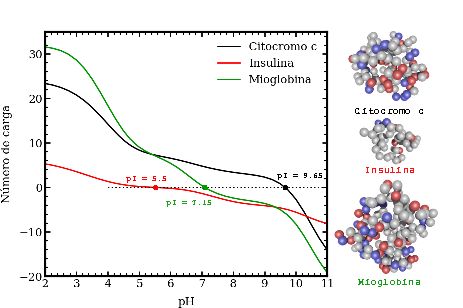
\includegraphics[width=0.65\textwidth]{Figures/graphs-gel2/protein-model.pdf}
     \caption{Izquierda: N\'umero de carga de las prote\'inas en una soluci\'on diluida en funci\'on del pH (curvas s\'olidas);
     	los c\'irculos llenos marcan el punto isoel\'ectrico,
     	donde la carga neta de la prote\'ina es cero.
     	La representaci\'on de grano grueso de las prote\'inas se ilustra a la derecha, donde los residuos de amino\'acidos se representan mediante una esfera \'unica (rojo: \'acido; azul: b\'asico; gris: residuos de carga neutral).}
     \label{fig:esf:protein-charge}
 \end{figure}



%%%%%%%%%%%%%%%%%%%%%%%%%%%%%%%%%%%%%%%%%%%%%%%%%%
\subsection{Modelo Molecular: Nanogel}
%%%%%%%%%%%%%%%%%%%%%%%%%%%%%%%%%%%%%%%%%%%%%%%%%%

Adem\'as del modelo de prote\'ina presentado en la secci\'on anterior, necesitamos especificar un modelo molecular para describir la red que compone a nuestro nanogel. Este modelo debe proporcionar un conjunto representativo de configuraciones moleculares de la red polim\'erica. Una conformaci\'on particular de la red se da por la posici\'on espacial de todos sus segmentos.
La red del nanogel est\'a compuesta por cadenas polim\'ericas entrecruzadas de 25 segmentos de longitud. En total, esta red contiene 10054 segmentos. Cada segmento es una representaci\'on simplificada de una unidad neutra (VA), un mon\'omero \'acido/b\'asico (MAA/AH) o un segmento entrecruzante. La \ref{table:Coarse-grain} incluye el volumen y el pKa (si la unidad es titulable) utilizados para describir estas unidades simplificadas.

La red del nanogel posee una topolog\'ia tipo diamante, donde los segmetos entrecruzantes se colocan en la posici\'on original de los \'atomos de carbono. Los entrecruzantes se conectan a 4 cadenas polim\'ericas. La construcci\'on de esta red se realiz\'o en primera instancia por la traslaci\'on tridimencional de la celda unidad en donde todas las cadenas polim\'ericas se encuentran alargadas, como segunod paso se realiz\'o un corte esferico de radio $R_{cut}$ medido desde el centro de masa de la estrucutura. El valor de $R_{cut}$ se hace de tal manera de obtener aproximadamente 10000 segmentos en total. 

Originalmente, todas las cadenas polim\'ericas se  conectan a dos entrecruzantes, pero como resultado de este procedimiento, el corte esferico, algunascadenas resultan quedar colgando en la superficie de la red, es decir  conectadas a un solo entrecruzante. La mayor\'ia de estas cadenas \emph{colgantes} superficiales son m\'as cortas que 25 segmentos. En conjunto, estas cadenas contienen el 22\% del n\'umero total de segmentos. Para generar las diferentes conformaciones moleculares de la red del pol\'imero, se ha realizado simulaciones de din\'amica molecular usando GROMACS 5.1.2\cite{lindahl2001gromacs}.

 \begin{figure}[!htb]
     \centering
     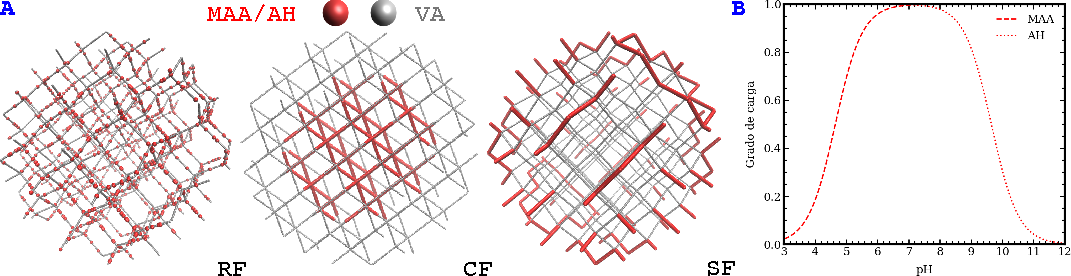
\includegraphics[width=0.99\textwidth]{Figures/graphs-gel2/ideal-charge-model.pdf}
     \caption{A: La red de nanogeles consiste en cadenas de copol\'imeros entrecruzadas con un segmento de carga neutral (VA: alcohol vin\'ilico) y una unidad funcional (ya sea MAA: \'acido metacr\'ilico o AH: alilamina).
     	Este esquema ilustra las tres distribuciones de de los comon\'omeros consideradas; de izquierda a derecha: RF: una distribuci\'on aleatoria de grupos funcionales en toda la red; CF: las unidades funcionales ocupan el centro/n\'ucleo de la red; SF: solo las cadenas colgantes libres en la superficie de la red est\'an funcionalizadas con unidades sensibles al pH.
     	B: Gr\'afico del grado de carga ideal dependiente del pH de la unidad funcional aislada en soluci\'on diluida.}
     \label{fig:esf:gel-topologies}
 \end{figure}


 
 
 Consideramos diferentes nanogeles sensibles al pH que contienen grupos \'acidos (MAA) o b\'asicos (AH), y evaluamos tres topolog\'ias diferentes para la distribuci\'on espacial de estos segmentos funcionales, que se esquematizan en la Figura \ref{fig:gel-topologies}:
 (i) una estructura \emph{aleatoriamente funcionalizada} (RF) donde los segmentos sensibles al pH se distribuyen aleatoriamente en toda la red,
 (ii) una estructura \emph{funcionalizada en el n\'ucleo} (CF), donde las unidades sensibles al pH ocupan el centro del nanogel, y
 (iii) una estructura \emph{funcionalizada en la superficie} (SF) en la cual solo las cadenas colgantes en la superficie de la red son ionizables.
  







%%%%%%%%%%%%%%%%%%%%%%%%%%%%%%%%%%%%%%%%%%%%%%%%%%
\section{Resultados y discusi\'on}
%%%%%%%%%%%%%%%%%%%%%%%%%%%%%%%%%%%%%%%%%%%%%%%%%%






%%%%%%%%%%%%%%%%%%%%%%%%%%%%%%%%%%%%%%%%%%%%%%%%%%
\subsection{Caraterizaci\'on del nanogel}
%%%%%%%%%%%%%%%%%%%%%%%%%%%%%%%%%%%%%%%%%%%%%%%%%%

En esta primera instancia, examinaremos el comportamiento (la respuesta) de los nanogeles en funci\'on del pH en ausencia de prote\'inas.

Para cuantificar el tama\~no de un nanogel, utilizaremos el radio medio de la part\'icula, $R$, que se puede calcular utilizando la siguiente fórmula:
\begin{align}
	R = \frac{4}{3}\frac{\int_0^\infty{dr\,G(r)\,r \left<\phi(r)\right>}}{\int_0^\infty{dr\,G(r)\left<\phi(r)\right>}}
\end{align}
\noindent donde $r$ es la distancia desde el centro de masa de la red polim\'erica ( como se ha mencionado en la sec. \ref{sec:esf:tm} se asume simetr\'ia radial);
$\left<\phi(r)\right>$ es la fracción de volumen local de la red polim\'erica;
los corchetes angulares indican el promedio de ensamble sobre las diferentes conformaciones de la red (ver ecuación \ref{eq:esf:ensamble-gel});
$G(r)=4\pi r^2$ es el \'area de la superficie de una esfera de radio $r$.

\begin{figure}[!htb]
     \centering
     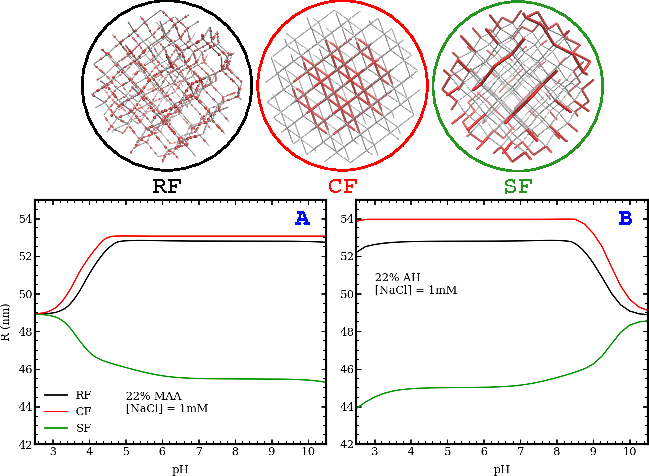
\includegraphics[width=0.9\textwidth]{Figures/graphs-gel2/rr-nano-pH.pdf}
     \caption{Radio promedio, R, en funci\'on del pH para nanogeles de copol\'imero MAA-VA (panel A) y AH-VA (panel B).
     	Se consideran tres estructuras diferentes en cada caso donde las unidades funcionales (MAA/AH) se distribuyen aleatoriamente a lo largo de la red polim\'erica (RF), ocupan el centro de la red (CF), o modifican las cadenas colgantes dentro del pol\'imero. interfaz de soluci\'on (SF).
     	En todos los casos, el $22\%$ de los segmentos de estas redes son sensibles al pH; La concentraci\'on de NaCl es $10^{-3}M$.}
     \label{fig:esf:gel-charge-MAA-AH}
\end{figure}


La Figura \ref{fig:esf:gel-charge-MAA-AH} muestra la relaci\'on entre el radio promedio ($R$) y el pH para tres estructuras diferentes: RF, CF y SF. En el panel A, se describe un nanogel con segmentos ionizables de $MAA$, mientras que en el panel B se presenta un nanogel basado en $AH$. En ambos casos, la concentraci\'on de sal es de 1 mM y la fracci\'on de mon\'omero funcional ($MAA$ o $AH$) es del $22\%$. Los nanogeles basados en $MAA$, funcionalizados al azar (RF) y en el n\'ucleo (CF), se hinchan a medida que aumenta el pH (panel A). Esto se debe a que los segmentos $MAA$ se desprotonan y adquieren carga el\'ectrica a medida que el pH aumenta (ver Figura \ref{fig:esf:gel-topologies}B), lo que resulta en repulsiones electrost\'asticas dentro de la red. Para reducir estas interacciones repulsivas, la distancia entre las unidades cargadas de $MAA$ debe aumentar, lo que provoca un aumento en el tama\~no de la red para separar estos segmentos cargados. En resumen, la expansi\'on neta de la red ocurre debido al aumento de la distancia espacial entre las unidades cargadas de $MAA$, como resultado de la necesidad de disminuir la repulsi\'on entre ellas.



Por otro lado, la red funcionalizada en su superficie con $MAA$ muestra un comportamiento de expansi\'on completamente diferente, como se puede observar en la Figura \ref{fig:esf:gel-charge-MAA-AH}A. Este nanogel se deshincha a medida que las unidades titulables se cargan al aumentar el pH. Para explicar este comportamiento contrario a lo esperado, hemos examinado la distribuci\'on local de segmentos dentro de nuestras estructuras en diferentes condiciones. Hemos utilizado la distribuci\'on radial de los mon\'omeros funcionales para los nanogeles $MAA$. Esta cantidad se define como:



%
\begin{align}
    \lambda_{MAA}(r)= 4\pi r^2\left<\phi^{MAA}(r)\right>
\end{align}
%
\noindent en donde $\left<\phi_{MAA}(r)\right>$ da la fracci\'on de volumen local de los segmentos de \'acido metacr\'ilico (ver ecuaci\'on \ref{eq:esf:ensamble-gel})
Hay que tener en cuenta que $\lambda_{MAA}(r) dr$ da el n\'umero de segmentos MAA en la capa esf\'erica entre $r$ y $r+dr$ medidos desde el centro del nanogel.
Adem\'as, la integral $\int_0^\infty \lambda_{MAA}(r) dr$ da el n\'umero total de mon\'omeros MAA en la red.


\begin{figure}[!htb]
     \centering
     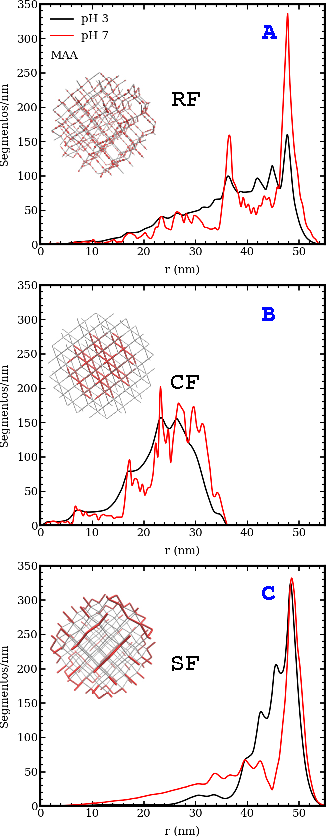
\includegraphics[width=0.45\textwidth]{Figures/graphs-gel2/dist-MAA.pdf}
     \caption{Distribuci\'on radial de segmentos MAA, $\lambda_{MAA}(r)$, a pH 3 y 7, y $10^{-3}M$ NaCl; cada panel corresponde a un nanogel de  MAA-VA diferente que tienen una funcionalizaci\'on de red particular y 22\% MAA.
     	Estos grupos funcionales est\'an completamente protonados (sin carga) a pH 3 y completamente disociados (cargados) a pH 7.}
     \label{fig:esf:MAA-vs-r-distribution}
 \end{figure}
 %\FloatBarrier

La Figura \ref{fig:esf:MAA-vs-r-distribution} muestra la distribuci\'on radial de los segmentos de MAA para las diferentes redes consideradas. En cada caso, se incluyen resultados para una soluci\'on de pH 3, donde los segmentos $MAA$ tienen carga neutra, y pH 7, donde est\'an completamente cargados (ver Figura \ref{fig:esf:gel-topologies}B). Para una funcionalizaci\'on de tipo aleatoria (Panel A), la distribuci\'on de los segmentos $MAA$ se desplaza hacia la interfaz de soluci\'on del nanogel a medida que la red se carga el\'ectricamente al aumentar el pH. Este desplazamiento ocurre para reducir las repulsiones electrost\'aticas entre los segmentos $MAA$ cargados.

Como resultado, toda la distribuci\'on del pol\'imero tambi\'en se extiende, incluidas las unidades $VA$ de carga neutra (ver Figura \ref{fig:esf:allr-distribution}). El mismo comportamiento tiene lugar para una funcionalizaci\'on central (Panel B), aunque por dise\~no, los segmentos $MAA$ en esta red, ya sea que est\'en cargados o no, es m\'as probable que ocurran a distancias m\'as cortas del centro del nanogel en comparaci\'on con las otras estructuras. El desplazamiento de segmentos a valores m\'as altos de r observado en los paneles A y B de la Figura \ref{fig:esf:MAA-vs-r-distribution} explica el aumento del tama\~no promedio del nanogel con pH observado en la Figura \ref{fig:esf:gel-charge-MAA-AH}A para las estructuras RF y CF.

Por otro lado, la Figura \ref{fig:esf:MAA-vs-r-distribution}C muestra que la distribuci\'on superficial de segmentos de $MAA$ se desplaza hacia el interior cuando la red se carga con el aumento de pH. Para reducir las repulsiones dentro de la red, las cadenas libres (de la superficie) de PMAA, que se asientan en la superficie del nanogel a un pH bajo, tambi\'en intentan ocupar el volumen dentro de la red cuando est\'an cargadas. Este cambio hacia el interior de la distribuci\'on de segmentos de pol\'imero (Figura \ref{fig:esf:allr-distribution}C) explica el comportamiento de deshinchamiento del nanogel tipo SF con el aumento del pH observado en la Figura \ref{fig:esf:gel-charge-MAA-AH}A. N\'otese, sin embargo, que a pesar de este desplazamiento parcial hacia el interior de la red, la posici\'on m\'as probable de los segmentos $MAA$ siempre es la interfaz pol\'imero-soluci\'on para soluciones de pH alto y bajo. Al empujar toda la estructura hacia el interior del nanogel, los segmentos de MAA quedan igualmente expuestos.





El comportamiento de los nanogeles compuestos por $AH$ es an\'alogo al de las redes basadas en $MAA$, pero en respuesta al cambio de pH en la direcci\'on opuesta.
Los grupos $AH$ se protonan y se cargan positivamente con la disminuci\'on del pH (ver figura \ref{fig:esf:gel-topologies}B).
Para nanogeles de $AH$ funcionalizados aleatoriamente y en su n\'ucleo, este aumento en la carga el\'ectrica con la disminución del pH provoca un desplazamiento hacia afuera de la distribuci\'on del segmento. Del mismo modo que se observ\'o para los nangoles compuestos por $MAA$% (ver \cref*{fig:AHseg_si}A y B)
, lo que explica la hinchaz\'on de la figura \ref{fig:esf:gel-charge-MAA-AH}B;
mientras tanto, para la estructuratipo SF, el deshinchamiento con la disminuci\'on del pH que se ve en la figura \ref{fig:esf:gel-charge-MAA-AH}B es consistente con un desplazamiento hacia adentro del pol\'imero %(ver \cref*{fig:AHseg_si}C) .


La figura \ref{fig:esf:allr-distribution} muestra la distribuci\'on de todos los segmentos que componen la red polim\'erica de los diferentes nanogeles. 
Al igual que en fig. \ref{fig:esf:MAA-vs-r-distribution} presentamos la distribuci\'pn para dos diferentes valores de pH. Que corresponde a los estados protonado (pH 3 ) y desprotonado (pH 7) de los segmentos de $MAA$.  En los paneles A y B se observa un aumento de cantidad de segmentos a valores m'as altos de $r$ al cargarse el nanogel. Comportamiento observado en la figura \ref{fig:esf:gel-charge-MAA-AH}, en donde hay un aumento del radio del nanogel (RF y CF).
En cambio el desplazamiento hacia dentro de los segmentos de la red polim\'erico al transicionar de un estado cargado a uno descargado en la distribuci\'on superficilal (SF) explica la disminuci\'on del tama\~no del gel observada en la figura \ref{fig:esf:gel-charge-MAA-AH}B.

El comportamiento de los nanogeles compuestos por AH es an\'alogo al de las redes basadas en $MAA$, pero en respuesta al cambio de pH en la direcci\'on opuesta. Los grupos AH se protonan y se cargan positivamente con la disminuci\'on del pH (ver Figura \ref{fig:esf:gel-topologies}B). Para nanogeles de AH funcionalizados aleatoriamente y en su n\'ucleo, este aumento en la carga el\'ectrica con la disminuci\'on del pH provoca un desplazamiento hacia afuera de la distribuci\'on del segmento, similar a lo observado para los nanogeles compuestos por MAA (ver Figura \ref{fig:AHseg_si}A y B). Esto explica la hinchaz\'on observada en la Figura \ref{fig:esf:gel-charge-MAA-AH}B. Por otro lado, para la estructura tipo SF, el deshinchamiento con la disminuci\'on del pH que se observa en la Figura \ref{fig:esf:gel-charge-MAA-AH}B es consistente con un desplazamiento hacia el interior del nanogel (ver Figura \ref{fig:AHseg_si}C).

Finalmente en la figura \ref{fig:esf:allr-distribution} se muestra la distribuci\'on de todos los segmentos que componen la red polim\'erica de los diferentes nanogeles (en este caso basados en $MAA$). Al igual que en la Figura \ref{fig:esf:MAA-vs-r-distribution}, presentamos la distribuci\'on para dos valores diferentes de pH, correspondientes a los estados protonado (pH 3) y desprotonado (pH 7) de los segmentos de $MAA$. En los paneles A y B se observa un aumento en la cantidad de segmentos a valores m\'as altos de $r$ a medida que el nanogel se carga. Este comportamiento es consistente con el aumento del radio del nanogel observado en la figura \ref{fig:esf:gel-charge-MAA-AH} para las estructuras RF y CF. Por otro lado, el desplazamiento hacia el interior de los segmentos de la red polim\'erica al transicionar de un estado cargado a uno descargado en la distribuci\'on superficial (SF) explica la disminuci\'on del tamañ\~no del nanogel observada en la figura \ref{fig:esf:gel-charge-MAA-AH}B.

\begin{figure}[!htb]
	\centering
	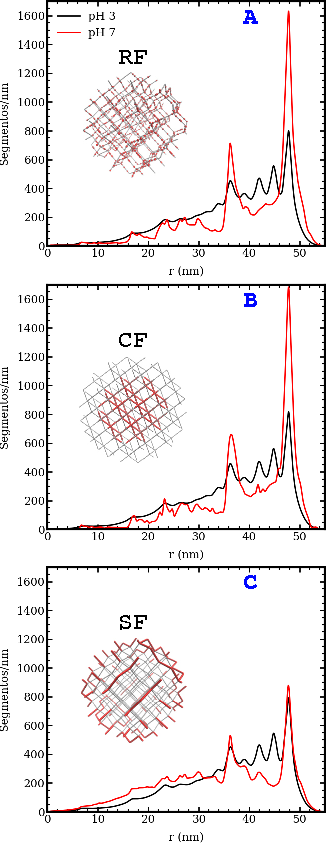
\includegraphics[width=0.45\textwidth]{Figures/graphs-gel2/allseg_SI.pdf}
	\caption{Distribuci\'on radial detodo los segmentos que componene la estructura del nanogel, $\lambda(r)$, a pH 3 y 7, y $10^{-3}M$ NaCl; cada panel corresponde a una funcionalizaci\'on  diferente}
	\label{fig:esf:allr-distribution}
\end{figure}




%%%%%%%%%%%%%%%%%%%%%%%%%%%%%%%%%%%%%%%%%%%%%%%%%%
\subsection{Adsorci\'on de prote\'inas en nanogeles basados en MAA}\label{sec:MAA-NGs}
%%%%%%%%%%%%%%%%%%%%%%%%%%%%%%%%%%%%%%%%%%%%%%%%%%



%%%%%%%%%%%%%%%%%%%%%%%%%%%
%%%%% Define Gamma and N(r)
%%%%%%%%%%%%%%%%%%%%%%%%%%%



En la secci\'on anterior, se evalu\'o el impacto de la funcionalizaci\'on de la red y la composici\'on qu\'imica en la respuesta del nanogel a las variaciones de pH en ausencia de prote\'inas. La reorganizaci\'on de los segmentos de la red polim\'erica es resultado de los cambios en el pH, con una dependencia en la elecci\'on de dise\~no, es decir, la distribuci\'on de unidades funcionales dentro de la red.

En esta parte, se mostrar\'a el impacto de esta reorganizaci\'on de la red polimé\'erica en el nivel de adsorci\'on de prote\'inas en diferentes nanogeles, as\'i como la distribuci\'on espacial de las prote\'inas adsorbidas. En particular, se presentar\'a el an\'alisis de la adsorci\'on del citocromo c y mioglobina en diferentes estructuras de nanogeles basados en $MAA$. Adem\'as, se realizar\'an estudios de adsorci\'on de insulina, pero en este caso con nanogeles que contienen $AH$ como segmento protonable. Los resultados de la insulina con MAA se omiten debido a su bajo punto isoel\'ectrico, ya que esta prote\'ina no se adsorbe en nanogeles basados en $MAA$.

Para estos estudios, se considerar\'a un nanogel polim\'erico centrado en $r=0$ en contacto con una soluci\'on acuosa de prote\'ina, con una concentraci\'on definida. El n\'umero de prote\'inas adsorbidas dentro de la capa esf\'erica entre $r$ y $r+dr$ se define como la cantidad en exceso. 
Definida como:


\begin{align}
     \langle N(r)\rangle dr = 4\pi r^2 \left(\langle\rho(r)\rangle - \rho_{bulk}\right) dr
\end{align}
%
en donde $\left<\rho(r)\right>$ y $\rho_{bulk}=\lim\limits_{r\to \infty } \langle\rho(r)\rangle$ son respectivamente la densidad (en n\'umero) local y en el bulk de la prote\'ina.
La integraci\'on de $\langle N(r)\rangle$ produce la \emph{adsorci\'on en exceso} (en adelante, simplemente la adsorci\'on) que cuantifica el n\'umero de prote\'inas incorporadas a la red de pol\'imeros,


%
\begin{align}
    \Gamma =  \int_0^\infty{  \langle N(r)\rangle dr}
\end{align}
%

%%%%%%%%%%%%%%%%%%%%%%%%%%%
%%%%% Adsorption to MAA NGs
%%%%%%%%%%%%%%%%%%%%%%%%%%%


\begin{figure}[!htb]
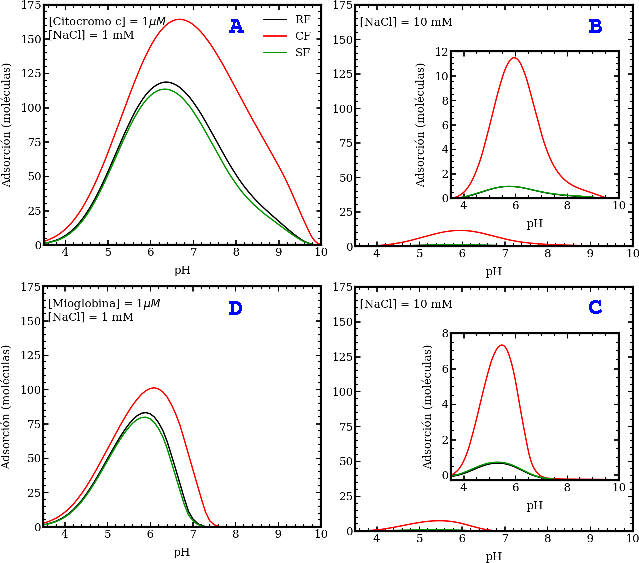
\includegraphics[width=0.9\textwidth]{Figures/graphs-gel2/ad-maa-pH-proteins.pdf}
\caption{Gr\'aficos del exceso de adsorci\'on $\Gamma$ de citocromo c (paneles A y B) y mioglobina (paneles C y D) a nanogeles MAA-VA en funci\'on del pH.
	La concentraci\'on de sal es $10^{-3}M$ en los paneles del lado izquierdo (A y C) y $10^{-2}M$ en los paneles del lado derecho
	(B y D); Se muestra una ampliaci'on de la adsorci\'on.
	Estos nanogeles tienen 22\% MAA; la concentraci\'on de prote\'ina es $10^{-6}M$.}
\label{fig:esf:adsorption-vs-pH-cyto-myo}
\end{figure}
 
 La Figura \ref{fig:esf:adsorption-vs-pH-cyto-myo} muestra la adsorci\'on de soluciones, de prote\'ina \'unica, de citocromo c (paneles superiores, A y B) y mioglobina (paneles inferiores, C y D) en nanogeles de MAA-VA con diferentes funcionalizaciones en su red. El pH se utiliz\'o como variable independiente en estos c\'alculos, y tambi\'en se evalu\'o el efecto de la concentraci\'on de NaCl al comparar diferentes paneles en la misma l\'inea. Los nanogeles de la Figura \ref{fig:esf:adsorption-vs-pH-cyto-myo} contienen un $22\%$ de MAA, lo que implica que todos los segmentos en las cadenas superficiales de la red est\'an compuestos por $MAA$.
 
 Se puede observar que la adsorci\'on de prote\'inas muestra un comportamiento no mon\'otono en funci\'on del pH, alcanzando un m\'aximo en la regi\'on entre pH 5 y 7. Este comportamiento est\'a influenciado por la concentraci\'on de sal y la prote\'ina espec\'ifica considerada. La respuesta de adsorci\'on al pH se puede explicar mediante las interacciones electrost\'aticas y el comportamiento de protonaci\'on de los segmentos de $MAA$ y las prote\'inas. A medida que el pH aumenta por encima del pKa intr\'inseco de $MAA$ ($4.65$), las unidades \'acidas del pol\'imero se disocian, cargando negativamente la red. Por encima del pKa, pero por debajo del punto isoel\'ectrico de las prote\'inas, estas adquieren carga positiva. En estas condiciones, las interacciones atractivas entre las prote\'inas y la red polim\'erica promueven la adsorci\'on de prote\'inas. Sin embargo, en ambos extremos de la escala de pH, estas interacciones son insignificantes: en pH bajo, el $MAA$ est\'a protonado y tiene carga neutra, mientras que en pH alto, las prote\'inas tienen carga negativa. En ambos casos, esto conduce a una ausencia de adsorci\'on ($\Gamma \approx 0$) o incluso a una desorci\'on ($\Gamma < 0$).
 
 
 
 
En general, las adsorciones de citocromo c y mioglobina son cualitativamente similares. Sin embargo, existen dos diferencias principales: (i) la magnitud de la adsorci\'on (el citocromo c se adsorbe significativamente m\'as) y (ii) el rango de pH en el que ocurre la adsorci\'on (el citocromo c se adsorbe en un rango de pH m\'as amplio debido a su punto isoel\'ectrico más alto, $9.65$ en comparaci\'on con $7.15$ para la mioglobina). Esto implica que, bajo condiciones similares, el nivel m\'aximo de adsorción de citocromo c se alcanza a un pH ligeramente m\'as alto.

En cuanto a las otras configuraciones, la Figura \ref{fig:esf:adsorption-vs-pH-cyto-myo} muestra que la distribuci\'on central de los segmentos $MAA$ conduce a una adsorci\'on significativamente mayor en la mayor\'ia de las condiciones. Demostramos que este comportamiento se debe a que dicha distribuci\'on de segmentos $MAA$ permite una incorporaci\'on m\'as efectiva de la prote\'ina adsorbida con carga el\'ectrica opuesta. Por otro lado, el comportamiento de adsorci\'on en las redes funcionalizadas aleatoriamente y en la superficie es sorprendentemente similar en el rango de pH y concentraciones de sal estudiadas, tanto para las diferentes prote\'inas como entre s\'i. Aunque las distribuciones de unidades funcionales entre las estructuras RF y SF difieren significativamente a pH bajo, se vuelven relativamente similares entre s\'i despu\'es de la reorganizaci\'on del nanogel a un pH m\'as alto cuando las unidades $MAA$ se cargan. Esto explica la adsorci\'on comparable de prote\'inas observada en los nanogeles RF y SF (compara los paneles A y C de la Figura \ref{fig:esf:MAA-vs-r-distribution}).



%%%%%%%%%%%%%%%%%%%%%%%%%%
%%%%% Protein localization
%%%%%%%%%%%%%%%%%%%%%%%%%%

\begin{figure}[!htb]
     \centering
     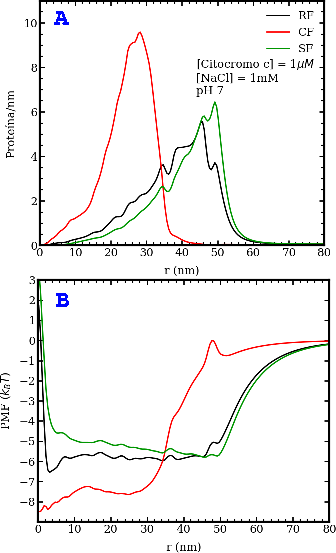
\includegraphics[width=0.45\textwidth]{Figures/graphs-gel2/cito-adsr-pmf.pdf}
     \caption{Panel A: Gr\'afico de la distribuci\'on radial de las mol\'eculas de citocromo c, $\langle N(r)\rangle$, en funci\'on de la posici\'on de los nanogeles MAA-VA con diferentes funcionalizaciones.
     	Estas redes tienen 22\% MAA, el pH es 7, la concentraci\'on de prote\'ina es de $10^{-6}M$ y la concentraci\'on de NaCl es de $10^{-3}M$.
     	El panel B muestra el potencial de la fuerza media, ${PMF}(r)$, que act\'ua sobre el citocromo c para las mismas condiciones que el panel A.}
     \label{fig:esf:adsorption-vs-r-cyto}
 \end{figure}



Para explicar el mejor rendimiento de los nanogeles MAA funcionalizados en su n\'ucleo en la incorporaci\'on de prote\'inas, se muestra en la Figura \ref{fig:esf:adsorption-vs-r-cyto}A la distribuci\'on radial de las mol\'eculas de citocromo c en funci\'on de la distancia $r$ al centro de masa del nanogel. La solución tiene un pH de 7 y una concentración de NaCl de $1 $ mM, que corresponde aproximadamente a las condiciones de m\'axima adsorci\'on de esta prote\'ina en la Figura \ref{fig:esf:adsorption-vs-pH-cyto-myo}A. Existe una clara correlaci\'on entre la distribuci\'on de los grupos funcionales a lo largo de la red polim\'erica y la ubicaci\'on del citocromo c adsorbido.

Cuando el n\'ucleo de la red est\'a funcionalizado, la mayor probabilidad de encontrar las prote\'inas ocurre en el interior del nanogel, entre 20 y 30 nm. En la figura \ref{fig:esf:adsorption-vs-r-cyto}A, el n\'umero m\'aximo de prote\'inas adsorbidas se produce a $r=28$ nm para 1 mM de NaCl, y a $r=25$ nm para 10 mM de NaCl. Coherentemente, el perfil de distribuci\'on de los grupos $MAA$ cargados muestra un m\'aximo suave en esta regi\'on espacial (ver Figura \ref{fig:esf:MAA-vs-r-distribution}B, curva roja). Es decir, las prote\'inas adsorbidas se ubican donde pueden estar rodeadas de segmentos de la red con carga el\'ectrica opuesta. Curiosamente, el mismo fen\'omeno ocurre en la adsorci\'on en los nanogeles RF y SF. Las distribuciones de MAA cargados muestran un m\'aximo pronunciado cerca de la superficie del nanogel, entre 45 y 50 nm (ver curvas rojas en la figura \ref{fig:esf:MAA-vs-r-distribution}, paneles A y C). La figura \ref{fig:esf:adsorption-vs-r-cyto}A muestra que el citocromo c es m\'as propenso a adsorberse junto a estas regiones de alta densidad de $MAA$ (carga).



Al comparar las distribuciones de citocromo c dentro de los nanogeles RF y SF en la Figura \ref{fig:esf:adsorption-vs-r-cyto}A, observamos que los perfiles son relativamente similares entre s\'i. Como era de esperar, si solo se funcionaliza la superficie, el perfil de la prote\'ina se desplaza hacia la interfaz pol\'imero-soluci\'on.

Para cuantificar a\'un m\'as la interacci\'on con los nanogeles, utilizamos el potencial de fuerza media (PMF) que act\'ua sobre una prote\'ina a una distancia $r$ desde el centro de la red polim\'erica. El PMF se define como:

\begin{align}
	\text{PMF}(r) = -k_B T \ln \frac{\langle \rho(r)\rangle}{\rho_{\text{bulk}}}
\end{align}

donde $\lim\limits_{r\to \infty}\text{PMF}(r)=0$, lo que indica que la interacci\'on nanogel-prote\'ina desaparece cuando est\'an separados.

La Figura \ref{fig:esf:adsorption-vs-r-cyto}B muestra el PMF que act\'ua sobre el citocromo c en las mismas condiciones que en el panel A, pero para las tres diferentes funcionalizaciones de nanogeles. En el interior del nanogel, la interacci\'on de la prote\'ina con la estructura CF es la m\'as fuerte, aproximadamente $-8k_B T$ en el rango espacial de $r=0$ a 30 nm. Esta interacci\'on es relativamente de corto alcance, ya que disminuye significativamente por encima de $r > 40$ nm.

Por otro lado, las interacciones del citocromo c con los nanogeles RF y SF se extienden m\'as lejos, hasta $55-60$ nm. En el interior del nanogel, estas interacciones son m\'as débiles que las de la estructura CF. La energ\'ia libre de adsorci\'on es aproximadamente $-6 k_BT$, y se mantiene aproximadamente constante dentro del nanogel RF.

Para el nanogel funcionalizado en la superficie, sin embargo, el m\'inimo del PMF tambi\'en es de alrededor de $-6 k_BT$, y ocurre junto a la interfaz pol\'imero-soluci\'on a $r\approx 50$ nm. A diferencia de la estructura RF, esta interacci\'on no es constante dentro del nanogel. 

En cambio, aumenta de manera mon\'otona a medida que $r$ disminuye, lo que indica que la prote\'ina se aleja de las cadenas superficiales funcionalizadas y se ubica m\'as profundamente en el nanogel.



%%%%%%%%%%
%%%% change in salt

\begin{figure}
     \centering
     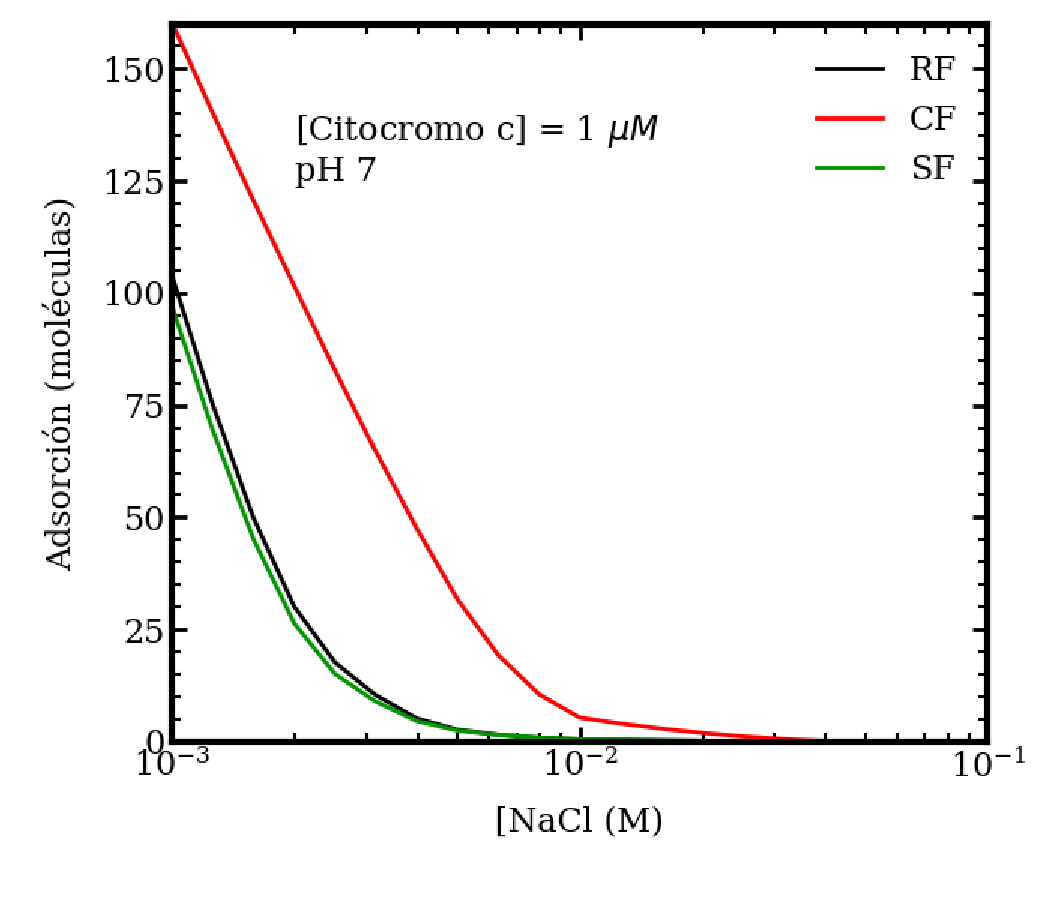
\includegraphics[width=0.45\textwidth]{Figures/graphs-gel2/gamma-salts-cito.pdf}
     \caption{Plot of the excess adsorption $\Gamma$ of cytochrome c as a function of salt concentration at pH 7 for MAA-VA nanogels with different network functionalizations having 22\% MAA; protein concentration is $10^{-6}M$.}
     \label{fig:esf:adsorption-vs-salt-cyto}
 \end{figure}
 

Una caracter\i'stica de la adsorci\'on de prote\'inas que nos falta discutir es el efecto de la concentraci\'on de sal.
Tanto para el citocromo c como para la mioglobina, la figura \ref{fig:esf:adsorption-vs-pH-cyto-myo} muestra que la incorporaci\'on de prote\'inas dentro de los diferentes nanogeles se ve significativamente mejorada al disminuir la concentraci\'on de sal en la soluci\'on.
Para caracterizar mejor este comportamiento, la figura \ref{fig:esf:adsorption-vs-salt-cyto} presenta la adsorci\'on de citocromo c en funci\'on de la concentraci\'on de NaCl a pH 7.
Este gr\'afico muestra que todas las funcionalizaciones de la red presentan un comportamiento cualitativamente similar, con una disminuci\'on dr\'astica en la adsorci\'on entre 1 y 10 mM de NaCl.
A 100 mM, todos los nanogeles muestran una adsorci\'on despreciable o negativa.

Cuando la concentraci\'on de sal en la soluci\'on es alta, tanto los iones Na$^+$ como los iones Cl$^-$ se encuentran en altas concentraciones dentro del nanogel.
Estos iones opacan las atracciones electrost\'aticas entre las cargas positivas de la prote\'ina y las cargas negativas del nanogel, que son la fuerza impulsora para la adsorci\'on de prote\'inas.
En efecto, estas atracciones se vuelven de corto alcance y no son lo suficientemente fuertes como para dar lugar a una adsorci\'on significativa, si es que ocurre.
Por otro lado, si la concentraci\'on de NaCl es menor, estas interacciones electrost\'aticas se ven menos apantalladas y efectivamente tienen un alcance mayor, lo que permite la adsorci\'on de prote\'inas.
Por lo tanto, la disminuci\'on de la concentraci\'on de sal mejora la adsorci\'on.
Este comportamiento ha sido observado en experimentos; los brushes de  polielectrolíticos muestran un aumento en la adsorci\'on de prote\'inas a baja concentraci\'on de sal \addcite[wittemann2006interaction,becker2012proteins, henzler2010adsorption,xu2018interaction].

Al considerar veh\'iculos para aplicaciones de liberaci\'on de prote\'inas, nuestros resultados sugieren que las mejores condiciones para la encapsulaci\'on corresponden a una baja concentraci\'on de sal.
Los perfiles de adsorci\'on de la Figura \ref{fig:esf:adsorption-vs-salt-cyto} son cualitativamente similares para las tres funcionalizaciones, pero el n\'umero de prote\'inas dentro del nanogel siempre es significativamente mayor para la estructura CF.
Esta caracter\'istica puede ser cr\'itica en el dise\~no de veh\'iculos de liberaci\'on para un objetivo que tenga una concentraci\'on de sal intermedia.
El CF incorpora m\'as prote\'inas en las mismas condiciones, pero puede no ser capaz de liberarlas si el objetivo tiene una concentraci\'on de sal intermedia.
Para estas condiciones, la funcionalizaci\'on aleatoria podr\'a liberar toda su carga.



%%%%%%%%%%%%%%%%%%%%%%%%%%%%%%%%%%%%%%%%%%%%%%%%%%
\subsection{Adsorci\'on de insulina en nanogeles basados en  AH} 
%%%%%%%%%%%%%%%%%%%%%%%%%%%%%%%%%%%%%%%%%%%%%%%%%%

La insulina no se adsorbe a los nanogeles de MAA de la secci\'on \ref{sec:MAA-NGs} %(ver \cref*{fig:adsoprtion-vs-pH-insulinMAA_si} en SI).
Esto se debe a que el punto isoel\'ectrico de la insulina y el pKa del $MAA$ est\'an cerca entre s\'i (numericamente hablando 5.5 y 4.65 respectivamente), lo que significa que para soluciones donde la prote\'ina tiene carga positiva, el nanogel tiene carga neutra, y si el nanogel tiene carga negativa, tambi\'en la tiene la prote\'ina.
En este contexto, decidimos investigar la adsorci\'on de insulina en un nanogel de alilamina, que tiene carga positiva por debajo de su pKa de 9.5, superponi\'endose con el rango donde la insulina tiene carga negativa.
Aparte de los mon\'omeros funcionales, la estructura de estas redes de copol\'imero AH-VA es la misma que la de los nanogeles de MAA-VA descritos anteriormente.


\begin{figure}[!htb]
    \centering
    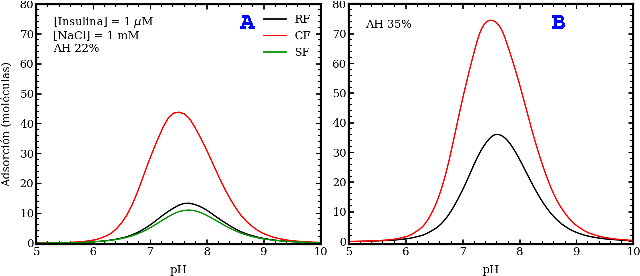
\includegraphics[width=0.9\textwidth]{Figures/graphs-gel2/insu-PAH.pdf}
    \caption{Plots of adsorbed insulin molecules, $\Gamma$, as a function of pH for  AH-VA nanogels having different functionalizations.
    The AH content is 22\% for the polymer networks of panel A and 35\% for those of panel B (this latter degree of functionalization cannot be achieved for the SF nanogel).
    Other conditions are $10^{-3}$\,M NaCl, and [Insulin] = $10^{-6}$\,M.}
    \label{fig:esf:adsorption-vs-pH-insulin}
\end{figure}




La figura \ref{fig:esf:adsorption-vs-pH-insulin}A muestra la adsorci\'on de insulina en nanogeles basados en AH con diferentes funcionalizaciones espaciales.
Una vez m\'as, hemos considerado redes con un $22\%$ de mon\'omeros sensibles al pH para poder incluir resultados para el nanogel SF, cuyas cadenas colgantes estan completamente compuestas  de $AH$
Las principales caracter\'isticas de este gr\'afico son cualitativamente similares a las de la adsorci\'on de citocromo c y mioglobina en los nanogeles de $MAA$ (ver figura \ref{fig:esf:adsorption-vs-pH-cyto-myo}).
Es decir, la insulina muestra una adsorci\'on no mon\'otona en función del pH de la soluci\'on.
Adem\'as, observamos que la distribuci\'on central de los segmentos de AH captura m\'as insulina que las funcionalizaciones aleatorias o superficiales.
Los nanogeles RF y SF muestran perfiles de adsorci\'on dependientes del pH relativamente similares.
Finalmente, una mayor concentraci\'on de sal tiene un efecto cr\'itico en la magnitud de la adsorci\'on de insulina, que disminuye significativamente debido al aumento del apantallamiento de las atracciones electrost\'aticas entre la red y la prote\'ina por los iones m\'oviles
%(las curvas de adsorción para $10^{-2}$,M de NaCl se pueden ver en la figura \ref{fig:esf:adsoprtion-AH-1d-2-insu_si}).

La figura \ref{fig:esf:adsorption-vs-pH-insulin}A muestra que los nanogeles basados en $AH$ son efectivos para encapsular insulina.
Sin embargo, a pesar de las similitudes cualitativas entre los perfiles de adsorci\'on de esta figura y los de citocromo c y mioglobina (\ref{fig:esf:adsorption-vs-pH-cyto-myo}A y C), vemos que la cantidad de mol'eculas de insulina capturadas por los nanogeles de $AH$ es significativamente menor que la de las otras prote\'inas capturadas por los nanogeles basados en $MAA$.
Por esta raz\'on, tambi\'en hemos evaluado el efecto del grado de funcionalizaci\'on de la red de pol\'imero para mejorar la adsorci\'on de prote\'inas.
La figura \ref{fig:esf:adsorption-vs-pH-insulin}B presenta la adsorci\'on de insulina para nanogeles con un $35\%$ de segmentos de AH.
En este caso, la estructura funcionalizada en la superficie no se incluye porque no hay suficientes segmentos en las cadenas para llegar a ese porcentaje.
Un mayor contenido de $AH$ promueve una mayor adsorci\'on, como se puede observar al comparar ambos paneles de la figura \ref{fig:esf:adsorption-vs-pH-insulin}.
Una vez m\'as, el nanogel CF adsorbe m\'as insulina que la red RF (m\'as del doble de prote\'inas para las condiciones de estos c\'alculos).




\begin{figure}[!htb]
    \centering
    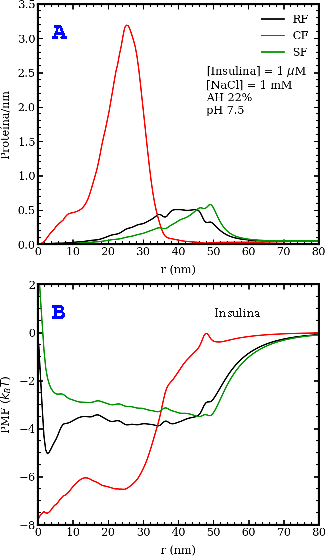
\includegraphics[width=0.45\textwidth]{Figures/graphs-gel2/insu-ads-pmf.pdf}
    \caption{A: Plot of the local distribution of insulin molecules, $\langle N(r)\rangle$, as a function of position for AH-VA nanogels having 22\% pH-sensitive segments in different network configurations.
    pH is 7.5, $10^{-6}$\,M insulin and  $10^{-3}$\,M NaCl.
    B: Potential of mean force,  ${PMF}(r)$, as a function of position for the same conditions as panel A.}
    \label{fig:esf:adsorption-vs-r-insulin}
\end{figure}



A continuaci\'on, describimos la distribuci\'on de mol\'eculas de insulina dentro de los nanogeles basados en AH.
La figura \ref{fig:esf:adsorption-vs-r-insulin}A muestra c\'omo se disponen espacialmente las prote\'inas adsorbidas dentro de los diferentes nanogeles basados en $AH$ con un grado de funcionalizaci\'on del $22\%$;
utilizamos ese grado de funcionalizaci\'on para comparar los resultados de los nanogeles CF, RF y SF.
El pH de estos resultados corresponde al m\'aximo de adsorci\'on de la figura \ref{fig:esf:adsorption-vs-pH-insulin}A.
La adsorci\'on de insulina en el nanogel CF no solo es significativamente mayor que la adsorci\'on en los nanogeles RF y SF, sino que tambi\'en ocurre en una posici\'on m\'as profunda dentro de la estructura.
La posici\'on m\'as probable de una mol\'ecula de insulina se encuentra alrededor de $r=25$,nm para el nanogel CF,
mientras que esta posici\'on se desplaza a alrededor de 40-45 y 50,nm para las estructuras RF y SF, respectivamente.

Para los nanogeles basados en MAA, la figura \ref{fig:esf:adsorption-vs-r-cyto}A muestra diferencias relativamente menores entre las distribuciones de citocromo c en los nanogeles RF y SF.
Estas diferencias se acent\'uan ligeramente al observar la adsorci\'on de insulina en los nanogeles AH-VA, como se muestra en la figura \ref{fig:esf:adsorption-vs-r-insulin}A.
La distribuci\'on de insulina se desplaza hacia el interior de la red en el nanogel modificado aleatoriamente en comparaci\'on con la funcionalizaci\'on superficial, donde las prote\'inas tienen m\'as probabilidades de ocupar la vecindad inmediata de la interfaz nanogel-soluci\'on.
Los perfiles de distribuci\'on de insulina siguen siendo relativamente similares para estas dos estructuras.

El panel B de la figura \ref{fig:esf:adsorption-vs-r-insulin} muestra el potencial de fuerza media que act\'ua sobre las mol\'eculas de insulina en las mismas condiciones que el panel A.
La interacci\'on atractiva en la insulina adsorbida var\'ia desde $-8$ hasta $-6 k_B T$ en el interior de la estructura CF y desde $-5$ hasta $-4 k_B T$ en el nanogel RF.
En el nanogel SF, el potencial presenta un m\'inimo de $-4 k_B T$ en la superficie y luego aumenta mon\'otonamente a medida que $r$ disminuye dentro del gel.
En general, los resultados de esta secci\'on muestran, una vez m\'as, que el dise\~no de la red (s\'intesis del nanogel) proporciona una herramienta para controlar la distribuci\'on de prote\'inas dentro del nanogel.






%%%%%%%%%%%%%%%%%%%%%%%%%%%%%%%%%%%%%%%%%%%%%%%%%%
\section{Conclusiones}
%%%%%%%%%%%%%%%%%%%%%%%%%%%%%%%%%%%%%%%%%%%%%%%%%%


Este cap\'itulo investigamos la adsorci\'n de prote\'inas en nanogeles de polim\'ericos con diferentes funcionalizaciones espaciales sensibles al pH. Se desarrolla y aplica nuestra teor\'iaa termodin\'amica basada en un modelo molecular.
El enfoque se centr\'o en la influencia de las interacciones electrost\'aticas, por lo cual se describieron tres prote\'inas con diferentes puntos isoel\'ectricos (insulina, mioglobina y citocromo c) utilizando un modelo molecular basado en sus estructuras cristalogr\'aficas.
Este studio explora las propiedades de los nanogeles sensibles al pH basados en \'acido metacrílico o monomeros de alilamina.
Se consideran tres configuraciones diferentes, con segmentos sensibles al pH distribuidos al azar, en el centro o en la superficie de la red del nanogel.

Se examin\'o el comportamiento de estos nanogeles en funci\'on del pH cuando no hay prote\'inas presentes en la soluci\'on.
Los resultados muestran que, para los nanogeles basados en \'acido metacr\'ilico, tanto los nanogeles distribuidos al azar como los funcionalizados en el n\'ucleo se hinchan con el aumento del pH, debido a la desprotonaci\'on y carga de los segmentos de \'acido metacr\'ilico, lo que conduce a repulsiones electrostá\'aicas intra-red.
Por otro lado, la red de \'acido metacr\'ilico funcionalizada en la superficie se deshincha a medida que las unidades titulables se cargan con el aumento del pH.
Este comportamiento contra intuitivo se puede explicar al observar la distribuci\'on local de los segmentos que componen la red dentro de estas estructuras en diferentes condiciones.
La reorganizaci\'on de la red del nanogel en respuesta a cambios en el pH depende de la funcionalizaci\'on espacial espec\'ifica.
Se realiz\'o el mismo an\'alisis para los nanogeles basados en alilamina y se obtuvieron resultados an\'alogos, con la direcci\'on de los est\'imulos invertida;
la diferencia clave radica en el comportamiento de sus unidades sensibles al pH: mientras que el \'acido metacr\'ilico es \'acido, la alilamina est\'a cargada a pH bajo y es neutra a pH alto.


Se evalu\'o la adsorci\'on de citocromo c y mioglobina en diferentes estructuras de nanogeles basados en MAA, y se encontr\'o que la adsorci\'on de prote\'inas es una funci\'on no mon\'otona del pH.
Los detalles cuantitativos de los perfiles de adsorci\'on dependen de la concentraci\'on de sal y de la prote\'ina espec\'ifica.
La respuesta al pH puede explicarse en t\'erminos de las interacciones electrost\'aticas y el comportamiento de protonaci\'on tanto de los segmentos de MAA como de los residuos de prote\'ina.
La reorganizaci\'on de los segmentos de las cadenas polim\'ericas en los nanogeles como resultado de los cambios de pH depende de la configuraci\'on espacial de las unidades funcionales dentro de la red, lo que tambi\'en regula el nivel y la localizaci\'on de las prote\'inas adsorbidas.
Tambi\'en hemos investigado la adsorci\'on de insulina en nanogeles de alilamina.
Nuestros resultados muestran que los nanogeles basados en AH son eficaces para encapsular insulina, y un mayor grado de funcionalizaci\'on resulta en una mayor adsorci\'on.

En el contexto del uso de nanogeles sensibles al pH para la liberaci\'on de prote\'inas, nuestros resultados enfatizan la importancia de considerar la distribuci\'on espacial de las unidades funcionales en la red de nanogeles durante la s\'intesis.
Este factor de dise\~no no solo afecta la respuesta mec\'anica macrosc\'opica del nanogel y su nivel de adsorci\'on de prote\'inas, sino que tambi\'en influye en la localizaci\'on de las prote\'inas adsorbidas dentro del nanogel.
La funcionalizaci\'on interna cerca del centro de la red polim\'erica conduce a una mayor encapsulaci\'on de prote\'inas, pero estos adsorbatos son menos accesibles para las interacciones superficiales con un objetivo.
Por otro lado, la distribuci\'on aleatoria de unidades sensibles al pH ofrece un mejor rendimiento si la entrega requiere interacciones prote\'ina-objetivo.
La funcionalizaci\'on superficial del nanogel proporciona una mejor disponibilidad de proteínas en la interfaz nanogel-objetivo, aunque potencialmente puede implicar una s\'intesis m\'as compleja.

La dependencia de la adsorci\'on de prote\'inas de la concentraci\'on de sal puede aprovecharse en el dise\~no de portadores funcionales para la entrega de prote\'inas.
Estos hallazgos indican que es mejor encapsular prote\'inas a bajas concentraciones de sal y liberarlas a altas concentraciones de sal, donde es menos probable que permanezcan en el nanogel.
Si el entorno objetivo tiene una concentraci\'on de sal intermedia, un nanogel con una distribuci\'on aleatoria de monomeros sensibles al pH es m\'as adecuado.
En conclusi\'on, los resultados de este cap\'itulo demuestran el papel cr\'itico que desempe\~na la funcionalizaci\'on de la red y la composici\'on qu\'imica en la determinaci\'on de la respuesta del nanogel a las variaciones de pH y la adsorci\'on de prote\'inas en estos nanogeles.
Esta informaci\'on es valiosa para el dise\~no de nanogeles sensibles al pH como veh\'iculos para la encapsulaci\'on, el transporte y la administraci\'on de prote\'inas.